\subsection{Fit Results}
\label{sec:FitResults}

Table \ref{tab:FitParams} shows the measured values for the extracted radii and scattering parameters, along with statistical and systematic error bars.
The "Fit Sys" and "Cut Sys" columns list the systematic uncertainties arising from variation in the fit method and in the topological and pair cut values, respectively.
In almost all cases, the cut systematics are an order of magnitude smaller than the fit method systematics.
The "Total Sys" column shows the fit method and cut systematics added in quadrature.


\begin{table}
\begin{center}

\begin{tabular}{|l|l|l|l|l|l|}
\hline 
Parameter & Value (fm) & $\pm$ Stat & $\pm$ Total Sys & Fit Sys & Cut Sys \\ 
\hline 
Radius $\Lambda\bar{\Lambda}$ 0-10\% & 2.9 & 0.3 & 0.3 & 0.3 & 0.02 \\ 
\hline 
Radius $\Lambda\bar{\Lambda}$ 10-30\%  & 2.3 & 0.2 & 0.2 & 0.2 & 0.02 \\ 
\hline 
Radius $\Lambda\bar{\Lambda}$ 30-50\%  & 1.8 & 0.2 & 0.2 & 0.2 & 0.01 \\ 
\hline 
Radius $\Lambda\Lambda$ 0-10\% & 5.4 & 0.6 & 0.2 & 0.2 & 0.1 \\ 
\hline 
Radius $\Lambda\Lambda$ 10-30\% & 4.2 & 0.5 & 0.2 & 0.2 & 0.04 \\ 
\hline 
$\Re(f_0)$ $\Lambda\bar{\Lambda}$ & -0.5 & 0.1 & 0.1 & 0.1 & 0.01 \\ 
\hline 
$\Im(f_0)$ $\Lambda\bar{\Lambda}$ & 0.14 & 0.09 & 0.02 & 0.02 & 0.006 \\ 
\hline 
$\Re(f_0)$ $\Lambda\Lambda$ & -0.6 & 0.3 & 0.05 & 0.04 & 0.02 \\ 
\hline 
$d_0$ $\Lambda\bar{\Lambda}$ & 1.7 & 0.2 & 0.2 & 0.2 & 0.01 \\ 
\hline 
$d_0$ $\Lambda\Lambda$ & 5.3 & 2.7 & 0.3 & 0.2 & 0.2 \\ 
\hline 
\end{tabular} 
\end{center}
\caption[Fit results]{Measured fit parameters with statistical and systematic errors.
All values are measured in fm.
The Fit Sys and Cut Sys columns show the systematic uncertainties arising from variations in the fit method and the topological and pair cut parameters, respectively.
The Total Sys column comes from the fit and cut systematic errors added in quadrature. }
\label{tab:FitParams}
\end{table}






\subsubsection{Discussion of results}
\label{sec:ResultsDiscussion}

Interpretation of final fit results will go here, along with comparisons to other results.

% Ref0

For the purpose of comparison, Figure \ref{fig:Ref0} shows the measured $\Re(f_0)$ for a number of different systems. From the left: $\Lambda\bar{\Lambda}$ and $\Lambda\Lambda \oplus \bar{\Lambda}\bar{\Lambda}$ scattering lengths from this analysis, $\Lambda\Lambda \oplus \bar{\Lambda}\bar{\Lambda}$ from Au--Au $\sqrt{s_{\mathrm{NN}}} = 200\ \mathrm{GeV}/c$ measured at STAR \cite{Adamczyk:2014vca}, $\Lambda\Lambda$ result from a 4-body cluster model of hypernuclear interactions \cite{Hiyama:2002yj} applied to a measurement of $\ce{^{6}_{\Lambda\Lambda}\mathrm{He}}$ \cite{Takahashi:2001nm}, $\Lambda\Lambda$ result from the Nijmegen D soft-core interaction model \cite{Filikhin:2002wm} (also applied to \cite{Hiyama:2002yj}), $\mathrm{p}\bar{\Lambda}$ extracted from a residual correlation analysis \cite{Kisiel:2014mma} of STAR data, $\mathrm{p}\Lambda$ singlet and triplet scattering lengths \cite{Wang:1999bf}, np singlet and triplet scattering lengths \cite{LANDAU1977502}, and the nn scattering length \cite{vonWitsch:1979uni}.

\begin{figure}[hbtp]
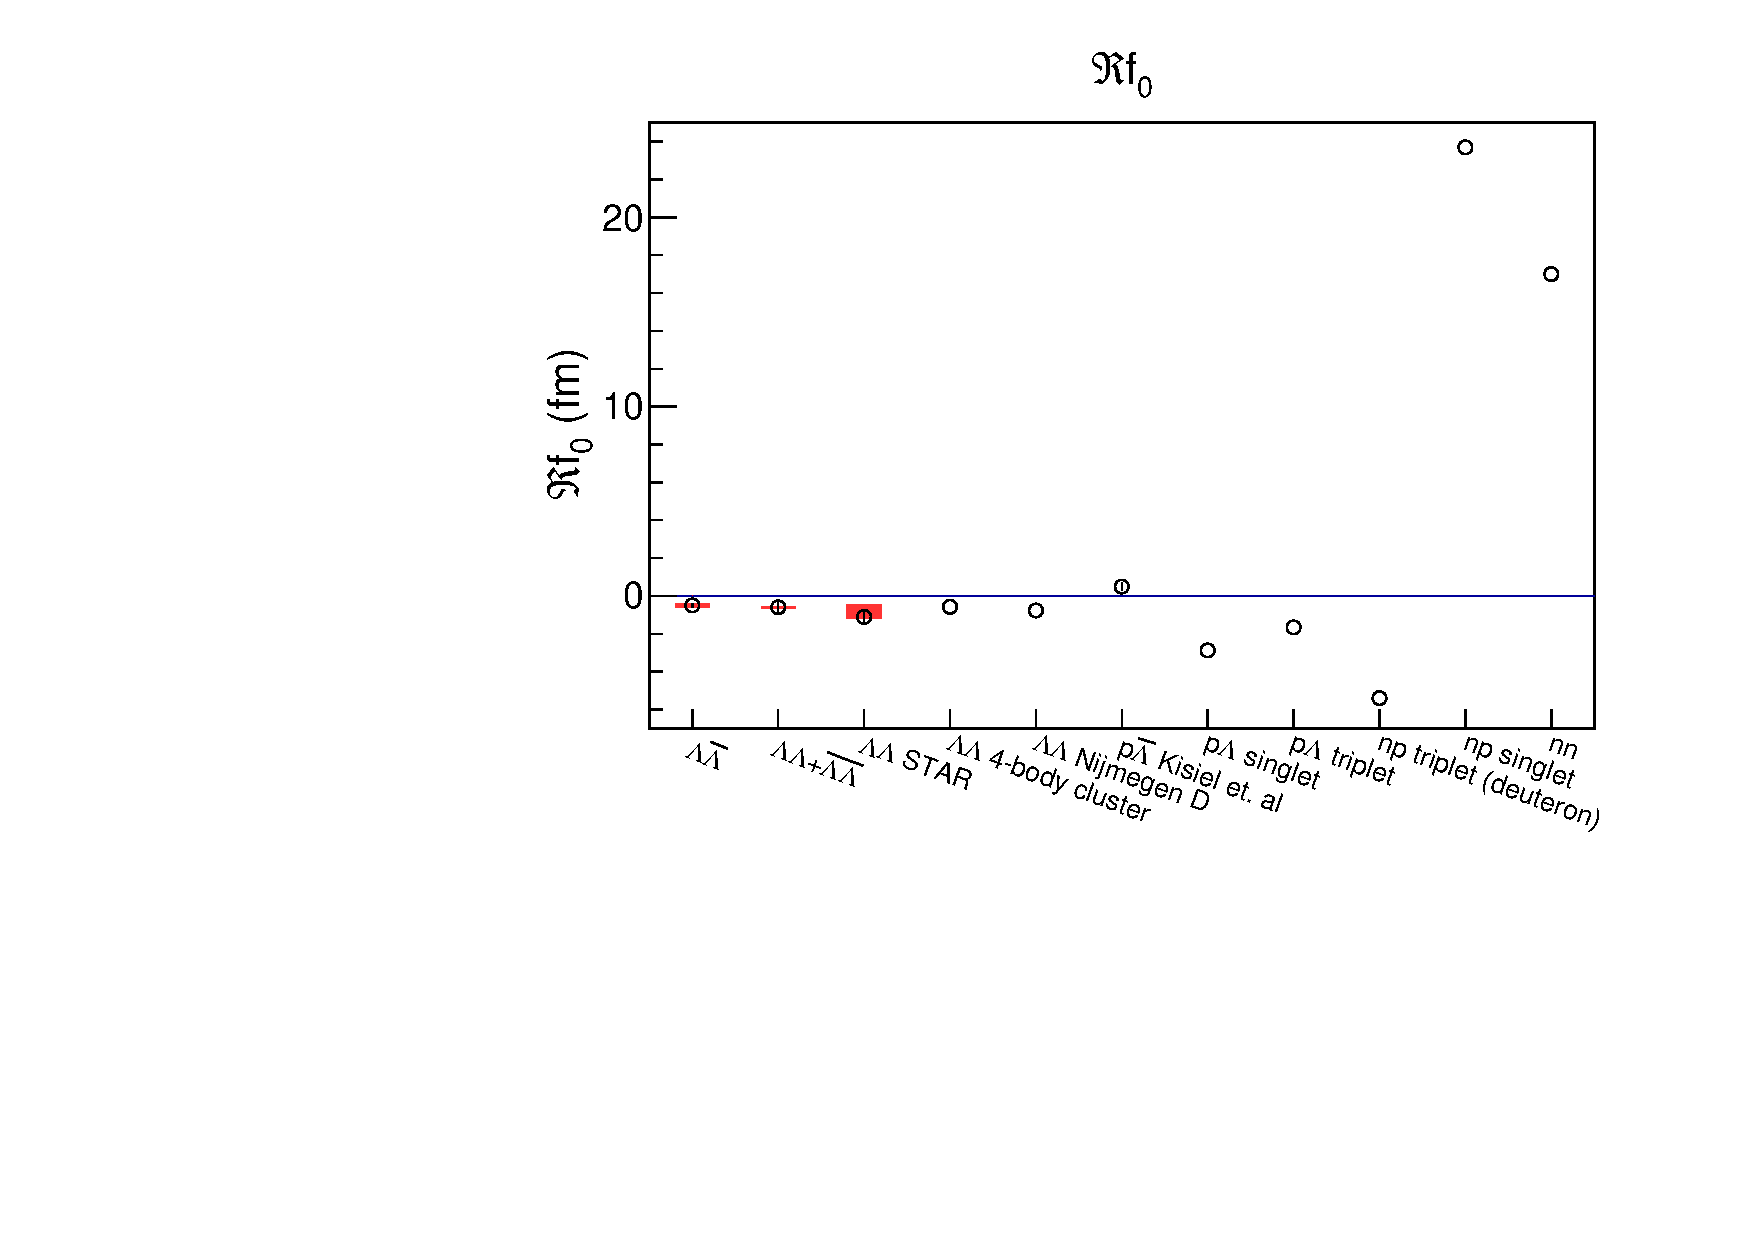
\includegraphics[width=36pc]{Figures/FitResults/2016-9-14-Ref0.pdf}
\caption[Measurements of $\Re(f_0)$ for various particle pairs]{Several measurements of the real part of the $\Lambda\Lambda$ and $\Lambda\bar{\Lambda}$ scattering lenghts. p$\Lambda$, p$\bar{\Lambda}$, np, and nn are included for comparison. The np spin-triplet state --- the deuteron --- is a weakly bound state. The $\Lambda\Lambda$ scattering length is an order of magnitude smaller than the np scattering length, which is evidence that there is no $\Lambda\Lambda$ dibaryon bound state.  }
\label{fig:Ref0}
\end{figure}

The np triplet spin state is a known bound state --- the ground state of the deuteron.
%  comparison with LL


% Zoomed in picture of the scattering lengths

% Imf0

% d0



% Add plot for ALICE mT scaling and scattering length comparisons

% Imf0 is small compared to ppbar and plambdabar.

